\documentclass{book}
\usepackage[a4paper,top=2.5cm,bottom=2.5cm,left=2.5cm,right=2.5cm]{geometry}
\usepackage{makeidx}
\usepackage{natbib}
\usepackage{graphicx}
\usepackage{multicol}
\usepackage{float}
\usepackage{listings}
\usepackage{color}
\usepackage{ifthen}
\usepackage[table]{xcolor}
\usepackage{textcomp}
\usepackage{alltt}
\usepackage{ifpdf}
\ifpdf
\usepackage[pdftex,
            pagebackref=true,
            colorlinks=true,
            linkcolor=blue,
            unicode
           ]{hyperref}
\else
\usepackage[ps2pdf,
            pagebackref=true,
            colorlinks=true,
            linkcolor=blue,
            unicode
           ]{hyperref}
\usepackage{pspicture}
\fi
\usepackage[utf8]{inputenc}
\usepackage{mathptmx}
\usepackage[scaled=.90]{helvet}
\usepackage{courier}
\usepackage{sectsty}
\usepackage{amssymb}
\usepackage[titles]{tocloft}
\usepackage{doxygen}
\lstset{language=C++,inputencoding=utf8,basicstyle=\footnotesize,breaklines=true,breakatwhitespace=true,tabsize=4,numbers=left }
\makeindex
\setcounter{tocdepth}{3}
\renewcommand{\footrulewidth}{0.4pt}
\renewcommand{\familydefault}{\sfdefault}
\hfuzz=15pt
\setlength{\emergencystretch}{15pt}
\hbadness=750
\tolerance=750
\begin{document}
\hypersetup{pageanchor=false,citecolor=blue}
\begin{titlepage}
\vspace*{7cm}
\begin{center}
{\Large M\-T }\\
\vspace*{1cm}
{\large Generated by Doxygen 1.8.3.1}\\
\vspace*{0.5cm}
{\small Sat May 11 2013 00:26:12}\\
\end{center}
\end{titlepage}
\clearemptydoublepage
\pagenumbering{roman}
\tableofcontents
\clearemptydoublepage
\pagenumbering{arabic}
\hypersetup{pageanchor=true,citecolor=blue}
\chapter{Namespace Index}
\section{Namespace List}
Here is a list of all documented namespaces with brief descriptions\-:\begin{DoxyCompactList}
\item\contentsline{section}{\hyperlink{namespacecmd}{cmd} \\*Command infrastructure namespace }{\pageref{namespacecmd}}{}
\end{DoxyCompactList}

\chapter{Hierarchical Index}
\section{Class Hierarchy}
This inheritance list is sorted roughly, but not completely, alphabetically\-:\begin{DoxyCompactList}
\item \contentsline{section}{central\-\_\-engine}{\pageref{classcentral__engine}}{}
\item \contentsline{section}{cmd\-:\-:cmd\-\_\-arg\-\_\-base}{\pageref{classcmd_1_1cmd__arg__base}}{}
\begin{DoxyCompactList}
\item \contentsline{section}{cmd\-\_\-arg\-\_\-bool}{\pageref{classcmd__arg__bool}}{}
\item \contentsline{section}{cmd\-\_\-arg\-\_\-double}{\pageref{classcmd__arg__double}}{}
\item \contentsline{section}{cmd\-\_\-arg\-\_\-int}{\pageref{classcmd__arg__int}}{}
\item \contentsline{section}{cmd\-\_\-arg\-\_\-string}{\pageref{classcmd__arg__string}}{}
\end{DoxyCompactList}
\item \contentsline{section}{cmd\-:\-:cmd\-\_\-base}{\pageref{classcmd_1_1cmd__base}}{}
\item \contentsline{section}{cmd\-:\-:cmd\-\_\-processor}{\pageref{classcmd_1_1cmd__processor}}{}
\item \contentsline{section}{cmd\-:\-:exception}{\pageref{classcmd_1_1exception}}{}
\end{DoxyCompactList}

\chapter{Class Index}
\section{Class List}
Here are the classes, structs, unions and interfaces with brief descriptions\-:\begin{DoxyCompactList}
\item\contentsline{section}{\hyperlink{classcentral__engine}{central\-\_\-engine} \\*Central engine to handle program initialization, uninitialization, command-\/line, e.\-t.\-c }{\pageref{classcentral__engine}}{}
\item\contentsline{section}{\hyperlink{classcmd_1_1cmd__arg__base}{cmd\-::cmd\-\_\-arg\-\_\-base} \\*Abstract base class for command args }{\pageref{classcmd_1_1cmd__arg__base}}{}
\item\contentsline{section}{\hyperlink{classcmd__arg__bool}{cmd\-\_\-arg\-\_\-bool} \\*Keeps boolean command argument }{\pageref{classcmd__arg__bool}}{}
\item\contentsline{section}{\hyperlink{classcmd__arg__double}{cmd\-\_\-arg\-\_\-double} \\*Keeps double command argument }{\pageref{classcmd__arg__double}}{}
\item\contentsline{section}{\hyperlink{classcmd__arg__int}{cmd\-\_\-arg\-\_\-int} \\*Keeps integer command argument }{\pageref{classcmd__arg__int}}{}
\item\contentsline{section}{\hyperlink{classcmd__arg__string}{cmd\-\_\-arg\-\_\-string} \\*Keeps string command argument }{\pageref{classcmd__arg__string}}{}
\item\contentsline{section}{\hyperlink{classcmd_1_1cmd__base}{cmd\-::cmd\-\_\-base} \\*Abstract base class commands }{\pageref{classcmd_1_1cmd__base}}{}
\item\contentsline{section}{\hyperlink{classcmd_1_1cmd__processor}{cmd\-::cmd\-\_\-processor} \\*Central singleton class for processing command line entries }{\pageref{classcmd_1_1cmd__processor}}{}
\item\contentsline{section}{\hyperlink{classcmd_1_1exception}{cmd\-::exception} \\*Exception system for cmd level exceptions }{\pageref{classcmd_1_1exception}}{}
\end{DoxyCompactList}

\chapter{File Index}
\section{File List}
Here is a list of all documented files with brief descriptions\-:\begin{DoxyCompactList}
\item\contentsline{section}{cmd\-\_\-arg/\hyperlink{cmd__arg__bool_8h}{cmd\-\_\-arg\-\_\-bool.\-h} \\*Definition of class \hyperlink{classcmd__arg__bool}{cmd\-\_\-arg\-\_\-bool} }{\pageref{cmd__arg__bool_8h}}{}
\item\contentsline{section}{cmd\-\_\-arg/\hyperlink{cmd__arg__double_8h}{cmd\-\_\-arg\-\_\-double.\-h} \\*Definition of class \hyperlink{classcmd__arg__double}{cmd\-\_\-arg\-\_\-double} }{\pageref{cmd__arg__double_8h}}{}
\item\contentsline{section}{cmd\-\_\-arg/\hyperlink{cmd__arg__int_8h}{cmd\-\_\-arg\-\_\-int.\-h} \\*Definition of class \hyperlink{classcmd__arg__int}{cmd\-\_\-arg\-\_\-int} }{\pageref{cmd__arg__int_8h}}{}
\item\contentsline{section}{cmd\-\_\-arg/\hyperlink{cmd__arg__string_8h}{cmd\-\_\-arg\-\_\-string.\-h} \\*Definition of class \hyperlink{classcmd__arg__string}{cmd\-\_\-arg\-\_\-string} }{\pageref{cmd__arg__string_8h}}{}
\item\contentsline{section}{cmd\-\_\-base/\hyperlink{cmd__arg__base_8cpp}{cmd\-\_\-arg\-\_\-base.\-cpp} \\*Definition of class cmd\-\_\-arg\-\_\-base }{\pageref{cmd__arg__base_8cpp}}{}
\item\contentsline{section}{cmd\-\_\-base/\hyperlink{cmd__arg__base_8h}{cmd\-\_\-arg\-\_\-base.\-h} \\*Declaration of class cmd\-\_\-arg\-\_\-base }{\pageref{cmd__arg__base_8h}}{}
\item\contentsline{section}{cmd\-\_\-base/\hyperlink{cmd__base_8cpp}{cmd\-\_\-base.\-cpp} \\*Definition of class cmd\-\_\-base }{\pageref{cmd__base_8cpp}}{}
\item\contentsline{section}{cmd\-\_\-base/\hyperlink{cmd__base_8h}{cmd\-\_\-base.\-h} \\*Declaration of class cmd\-\_\-base }{\pageref{cmd__base_8h}}{}
\item\contentsline{section}{cmd\-\_\-processor/\hyperlink{cmd__processor_8cpp}{cmd\-\_\-processor.\-cpp} \\*Definition of class cmd\-\_\-processor }{\pageref{cmd__processor_8cpp}}{}
\item\contentsline{section}{cmd\-\_\-processor/\hyperlink{cmd__processor_8h}{cmd\-\_\-processor.\-h} \\*Declaration of class cmd\-\_\-processor }{\pageref{cmd__processor_8h}}{}
\item\contentsline{section}{exceptions/\hyperlink{cmd__exception_8cpp}{cmd\-\_\-exception.\-cpp} \\*Definition of class exception }{\pageref{cmd__exception_8cpp}}{}
\item\contentsline{section}{exceptions/\hyperlink{cmd__exception_8h}{cmd\-\_\-exception.\-h} \\*Declaration of class exception }{\pageref{cmd__exception_8h}}{}
\item\contentsline{section}{main/\hyperlink{central__engine_8cpp}{central\-\_\-engine.\-cpp} \\*Definition of class \hyperlink{classcentral__engine}{central\-\_\-engine} }{\pageref{central__engine_8cpp}}{}
\item\contentsline{section}{main/\hyperlink{central__engine_8h}{central\-\_\-engine.\-h} \\*Declaration of class \hyperlink{classcentral__engine}{central\-\_\-engine} }{\pageref{central__engine_8h}}{}
\end{DoxyCompactList}

\chapter{Namespace Documentation}
\hypertarget{namespacecmd}{\section{cmd Namespace Reference}
\label{namespacecmd}\index{cmd@{cmd}}
}


command infrastructure namespace  


\subsection*{Classes}
\begin{DoxyCompactItemize}
\item 
class \hyperlink{classcmd_1_1cmd__arg__base}{cmd\-\_\-arg\-\_\-base}
\begin{DoxyCompactList}\small\item\em Abstract base class for command args. \end{DoxyCompactList}\item 
class \hyperlink{classcmd_1_1cmd__base}{cmd\-\_\-base}
\begin{DoxyCompactList}\small\item\em Abstract base class commands. \end{DoxyCompactList}\item 
class \hyperlink{classcmd_1_1cmd__processor}{cmd\-\_\-processor}
\begin{DoxyCompactList}\small\item\em Central singleton class for processing command line entries. \end{DoxyCompactList}\item 
class \hyperlink{classcmd_1_1exception}{exception}
\begin{DoxyCompactList}\small\item\em exception system for cmd level exceptions. \end{DoxyCompactList}\end{DoxyCompactItemize}


\subsection{Detailed Description}
command infrastructure namespace 
\chapter{Class Documentation}
\hypertarget{classcentral__engine}{\section{central\-\_\-engine Class Reference}
\label{classcentral__engine}\index{central\-\_\-engine@{central\-\_\-engine}}
}


Central engine to handle program initialization, uninitialization, command-\/line, e.\-t.\-c.  




{\ttfamily \#include $<$central\-\_\-engine.\-h$>$}

\subsection*{Program handling management}
\begin{DoxyCompactItemize}
\item 
\hypertarget{classcentral__engine_ad71abe717a7b00af96d485d9d20f03a5}{void \hyperlink{classcentral__engine_ad71abe717a7b00af96d485d9d20f03a5}{run} ()}\label{classcentral__engine_ad71abe717a7b00af96d485d9d20f03a5}

\begin{DoxyCompactList}\small\item\em Runs... \end{DoxyCompactList}\end{DoxyCompactItemize}
\subsection*{singleton management}
\begin{DoxyCompactItemize}
\item 
\hypertarget{classcentral__engine_a852875ee7b8279803b4c43d5988f51b0}{static \hyperlink{classcentral__engine}{central\-\_\-engine} \& \hyperlink{classcentral__engine_a852875ee7b8279803b4c43d5988f51b0}{get\-\_\-instance} ()}\label{classcentral__engine_a852875ee7b8279803b4c43d5988f51b0}

\begin{DoxyCompactList}\small\item\em Gets singletone object. \end{DoxyCompactList}\item 
\hypertarget{classcentral__engine_a44a4aa7379eb48e7dfb11909c361d740}{static void \hyperlink{classcentral__engine_a44a4aa7379eb48e7dfb11909c361d740}{instantiate} ()}\label{classcentral__engine_a44a4aa7379eb48e7dfb11909c361d740}

\begin{DoxyCompactList}\small\item\em Intstantiates singletone object. \end{DoxyCompactList}\item 
\hypertarget{classcentral__engine_ae8401a3e9da3b1ba124c4113b0f3fc02}{static void \hyperlink{classcentral__engine_ae8401a3e9da3b1ba124c4113b0f3fc02}{destroy} ()}\label{classcentral__engine_ae8401a3e9da3b1ba124c4113b0f3fc02}

\begin{DoxyCompactList}\small\item\em Destroys singletone object. \end{DoxyCompactList}\end{DoxyCompactItemize}
\subsection*{Special member functions.}
\begin{DoxyCompactItemize}
\item 
\hypertarget{classcentral__engine_a64c491c757e264a13d561421171c76bb}{\hyperlink{classcentral__engine_a64c491c757e264a13d561421171c76bb}{central\-\_\-engine} ()}\label{classcentral__engine_a64c491c757e264a13d561421171c76bb}

\begin{DoxyCompactList}\small\item\em Constructor. \end{DoxyCompactList}\item 
\hypertarget{classcentral__engine_a8dcca4e3b04a1f43b726b6fe79ee401f}{\hyperlink{classcentral__engine_a8dcca4e3b04a1f43b726b6fe79ee401f}{$\sim$central\-\_\-engine} ()}\label{classcentral__engine_a8dcca4e3b04a1f43b726b6fe79ee401f}

\begin{DoxyCompactList}\small\item\em Destructor. \end{DoxyCompactList}\end{DoxyCompactItemize}


\subsection{Detailed Description}
Central engine to handle program initialization, uninitialization, command-\/line, e.\-t.\-c. 

The documentation for this class was generated from the following files\-:\begin{DoxyCompactItemize}
\item 
main/\hyperlink{central__engine_8h}{central\-\_\-engine.\-h}\item 
main/\hyperlink{central__engine_8cpp}{central\-\_\-engine.\-cpp}\end{DoxyCompactItemize}

\hypertarget{classcmd_1_1cmd__arg__base}{\section{cmd\-:\-:cmd\-\_\-arg\-\_\-base Class Reference}
\label{classcmd_1_1cmd__arg__base}\index{cmd\-::cmd\-\_\-arg\-\_\-base@{cmd\-::cmd\-\_\-arg\-\_\-base}}
}


Abstract base class for command args.  




{\ttfamily \#include $<$cmd\-\_\-arg\-\_\-base.\-h$>$}

Inheritance diagram for cmd\-:\-:cmd\-\_\-arg\-\_\-base\-:\begin{figure}[H]
\begin{center}
\leavevmode
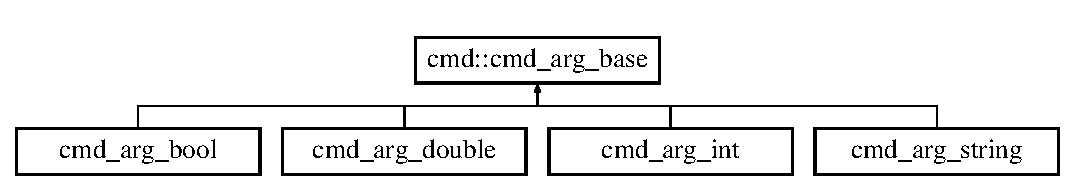
\includegraphics[height=2.000000cm]{classcmd_1_1cmd__arg__base}
\end{center}
\end{figure}
\subsection*{Public Member Functions}
\begin{DoxyCompactItemize}
\item 
\hypertarget{classcmd_1_1cmd__arg__base_a2f2b037e416eb71c4922e15637a459d9}{bool \hyperlink{classcmd_1_1cmd__arg__base_a2f2b037e416eb71c4922e15637a459d9}{is\-\_\-specified} () const }\label{classcmd_1_1cmd__arg__base_a2f2b037e416eb71c4922e15637a459d9}

\begin{DoxyCompactList}\small\item\em Returns true if argument is specified, otherwise returns false. \end{DoxyCompactList}\item 
void \hyperlink{classcmd_1_1cmd__arg__base_a6e2d899a1e0cb0a8babbcb2dceda7a85}{set\-\_\-specified} (bool s)
\begin{DoxyCompactList}\small\item\em Sets specified flag of argument. \end{DoxyCompactList}\item 
const std\-::string \& \hyperlink{classcmd_1_1cmd__arg__base_ab68609a393e1be2f50199a6af09ce107}{get\-\_\-name} () const 
\begin{DoxyCompactList}\small\item\em Gets argument's name. \end{DoxyCompactList}\item 
bool \hyperlink{classcmd_1_1cmd__arg__base_a217bfd2e37d9d45366e2ae649364f4e3}{is\-\_\-equal} (const std\-::string \&n) const 
\begin{DoxyCompactList}\small\item\em Checks if argument has same name. \end{DoxyCompactList}\item 
virtual void \hyperlink{classcmd_1_1cmd__arg__base_a2767ec77135f82eac5f3ca754b24acff}{set\-\_\-value} (const std\-::string \&v)=0
\begin{DoxyCompactList}\small\item\em Pure virtual function to set argument's value. \end{DoxyCompactList}\item 
\hypertarget{classcmd_1_1cmd__arg__base_a6d3b76394a6fb601e4e50cf349e60436}{virtual void \hyperlink{classcmd_1_1cmd__arg__base_a6d3b76394a6fb601e4e50cf349e60436}{reset} ()=0}\label{classcmd_1_1cmd__arg__base_a6d3b76394a6fb601e4e50cf349e60436}

\begin{DoxyCompactList}\small\item\em Pure virtual function to reset argument. \end{DoxyCompactList}\item 
\hyperlink{classcmd_1_1cmd__arg__base_a6a8a3cc24add61aa01748592cdd25798}{cmd\-\_\-arg\-\_\-base} (const std\-::string \&name)
\begin{DoxyCompactList}\small\item\em Constructor. \end{DoxyCompactList}\item 
\hypertarget{classcmd_1_1cmd__arg__base_a1322db06597ff12b16490bfdb62159cd}{virtual \hyperlink{classcmd_1_1cmd__arg__base_a1322db06597ff12b16490bfdb62159cd}{$\sim$cmd\-\_\-arg\-\_\-base} ()}\label{classcmd_1_1cmd__arg__base_a1322db06597ff12b16490bfdb62159cd}

\begin{DoxyCompactList}\small\item\em Virtual destructor. \end{DoxyCompactList}\end{DoxyCompactItemize}


\subsection{Detailed Description}
Abstract base class for command args. 

\subsection{Constructor \& Destructor Documentation}
\hypertarget{classcmd_1_1cmd__arg__base_a6a8a3cc24add61aa01748592cdd25798}{\index{cmd\-::cmd\-\_\-arg\-\_\-base@{cmd\-::cmd\-\_\-arg\-\_\-base}!cmd\-\_\-arg\-\_\-base@{cmd\-\_\-arg\-\_\-base}}
\index{cmd\-\_\-arg\-\_\-base@{cmd\-\_\-arg\-\_\-base}!cmd::cmd_arg_base@{cmd\-::cmd\-\_\-arg\-\_\-base}}
\subsubsection[{cmd\-\_\-arg\-\_\-base}]{\setlength{\rightskip}{0pt plus 5cm}cmd\-::cmd\-\_\-arg\-\_\-base\-::cmd\-\_\-arg\-\_\-base (
\begin{DoxyParamCaption}
\item[{const std\-::string \&}]{name}
\end{DoxyParamCaption}
)}}\label{classcmd_1_1cmd__arg__base_a6a8a3cc24add61aa01748592cdd25798}


Constructor. 


\begin{DoxyParams}{Parameters}
{\em name} & Name of Argument. \\
\hline
\end{DoxyParams}


\subsection{Member Function Documentation}
\hypertarget{classcmd_1_1cmd__arg__base_ab68609a393e1be2f50199a6af09ce107}{\index{cmd\-::cmd\-\_\-arg\-\_\-base@{cmd\-::cmd\-\_\-arg\-\_\-base}!get\-\_\-name@{get\-\_\-name}}
\index{get\-\_\-name@{get\-\_\-name}!cmd::cmd_arg_base@{cmd\-::cmd\-\_\-arg\-\_\-base}}
\subsubsection[{get\-\_\-name}]{\setlength{\rightskip}{0pt plus 5cm}const std\-::string \& cmd\-::cmd\-\_\-arg\-\_\-base\-::get\-\_\-name (
\begin{DoxyParamCaption}
{}
\end{DoxyParamCaption}
) const}}\label{classcmd_1_1cmd__arg__base_ab68609a393e1be2f50199a6af09ce107}


Gets argument's name. 

\begin{DoxyReturn}{Returns}
Constant access to argument name. 
\end{DoxyReturn}
\hypertarget{classcmd_1_1cmd__arg__base_a217bfd2e37d9d45366e2ae649364f4e3}{\index{cmd\-::cmd\-\_\-arg\-\_\-base@{cmd\-::cmd\-\_\-arg\-\_\-base}!is\-\_\-equal@{is\-\_\-equal}}
\index{is\-\_\-equal@{is\-\_\-equal}!cmd::cmd_arg_base@{cmd\-::cmd\-\_\-arg\-\_\-base}}
\subsubsection[{is\-\_\-equal}]{\setlength{\rightskip}{0pt plus 5cm}bool cmd\-::cmd\-\_\-arg\-\_\-base\-::is\-\_\-equal (
\begin{DoxyParamCaption}
\item[{const std\-::string \&}]{n}
\end{DoxyParamCaption}
) const}}\label{classcmd_1_1cmd__arg__base_a217bfd2e37d9d45366e2ae649364f4e3}


Checks if argument has same name. 


\begin{DoxyParams}{Parameters}
{\em n} & Name to compare. \\
\hline
\end{DoxyParams}
\begin{DoxyReturn}{Returns}
true if argument's name is equal to the given name. 
\end{DoxyReturn}
\hypertarget{classcmd_1_1cmd__arg__base_a6e2d899a1e0cb0a8babbcb2dceda7a85}{\index{cmd\-::cmd\-\_\-arg\-\_\-base@{cmd\-::cmd\-\_\-arg\-\_\-base}!set\-\_\-specified@{set\-\_\-specified}}
\index{set\-\_\-specified@{set\-\_\-specified}!cmd::cmd_arg_base@{cmd\-::cmd\-\_\-arg\-\_\-base}}
\subsubsection[{set\-\_\-specified}]{\setlength{\rightskip}{0pt plus 5cm}void cmd\-::cmd\-\_\-arg\-\_\-base\-::set\-\_\-specified (
\begin{DoxyParamCaption}
\item[{bool}]{s}
\end{DoxyParamCaption}
)}}\label{classcmd_1_1cmd__arg__base_a6e2d899a1e0cb0a8babbcb2dceda7a85}


Sets specified flag of argument. 


\begin{DoxyParams}{Parameters}
{\em s} & flag to set. \\
\hline
\end{DoxyParams}
\hypertarget{classcmd_1_1cmd__arg__base_a2767ec77135f82eac5f3ca754b24acff}{\index{cmd\-::cmd\-\_\-arg\-\_\-base@{cmd\-::cmd\-\_\-arg\-\_\-base}!set\-\_\-value@{set\-\_\-value}}
\index{set\-\_\-value@{set\-\_\-value}!cmd::cmd_arg_base@{cmd\-::cmd\-\_\-arg\-\_\-base}}
\subsubsection[{set\-\_\-value}]{\setlength{\rightskip}{0pt plus 5cm}virtual void cmd\-::cmd\-\_\-arg\-\_\-base\-::set\-\_\-value (
\begin{DoxyParamCaption}
\item[{const std\-::string \&}]{v}
\end{DoxyParamCaption}
)\hspace{0.3cm}{\ttfamily [pure virtual]}}}\label{classcmd_1_1cmd__arg__base_a2767ec77135f82eac5f3ca754b24acff}


Pure virtual function to set argument's value. 


\begin{DoxyParams}{Parameters}
{\em v} & Value to set. \\
\hline
\end{DoxyParams}


Implemented in \hyperlink{classcmd__arg__bool_a588134657e85b4ce161f5030f354f00d}{cmd\-\_\-arg\-\_\-bool}, \hyperlink{classcmd__arg__double_a4b7dc6e7a0520080f456896635eaaa1a}{cmd\-\_\-arg\-\_\-double}, \hyperlink{classcmd__arg__int_a04883e51fb34d7c2e3b9c6b6e3151ad8}{cmd\-\_\-arg\-\_\-int}, and \hyperlink{classcmd__arg__string_a434d6b2a9a6ae7e35043113cc0551140}{cmd\-\_\-arg\-\_\-string}.



The documentation for this class was generated from the following files\-:\begin{DoxyCompactItemize}
\item 
cmd\-\_\-base/\hyperlink{cmd__arg__base_8h}{cmd\-\_\-arg\-\_\-base.\-h}\item 
cmd\-\_\-base/\hyperlink{cmd__arg__base_8cpp}{cmd\-\_\-arg\-\_\-base.\-cpp}\end{DoxyCompactItemize}

\hypertarget{classcmd__arg__bool}{\section{cmd\-\_\-arg\-\_\-bool Class Reference}
\label{classcmd__arg__bool}\index{cmd\-\_\-arg\-\_\-bool@{cmd\-\_\-arg\-\_\-bool}}
}


Keeps boolean command argument.  




{\ttfamily \#include $<$cmd\-\_\-arg\-\_\-bool.\-h$>$}

Inheritance diagram for cmd\-\_\-arg\-\_\-bool\-:\begin{figure}[H]
\begin{center}
\leavevmode
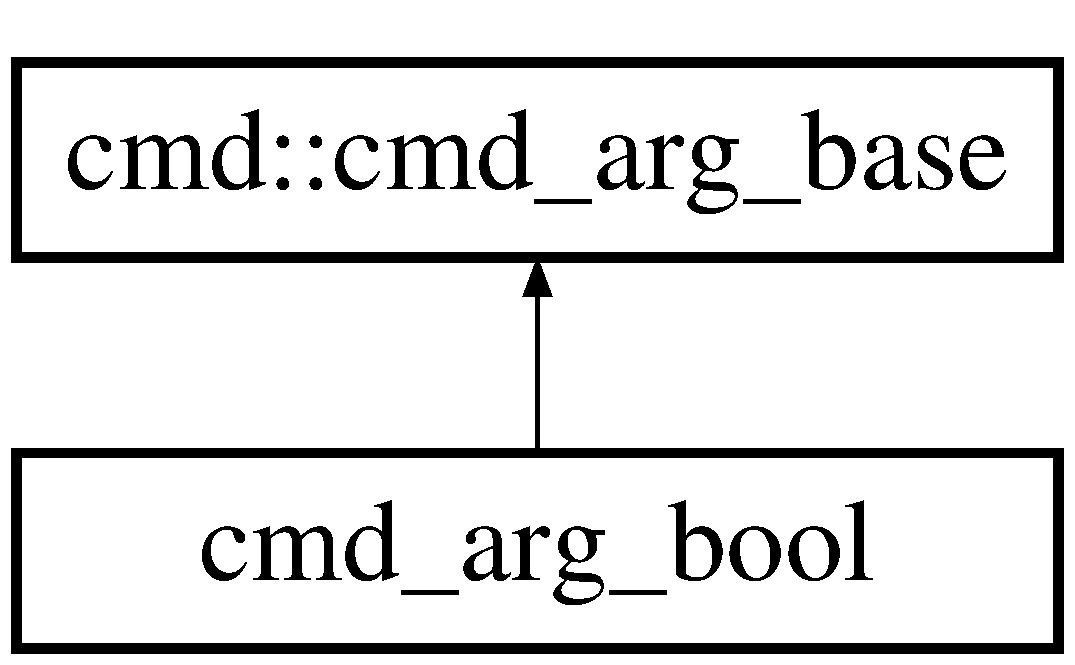
\includegraphics[height=2.000000cm]{classcmd__arg__bool}
\end{center}
\end{figure}
\subsection*{Public Member Functions}
\begin{DoxyCompactItemize}
\item 
\hypertarget{classcmd__arg__bool_a89c039485a3d0a7266c18ae1f414a7ff}{bool \hyperlink{classcmd__arg__bool_a89c039485a3d0a7266c18ae1f414a7ff}{get\-\_\-value} () const }\label{classcmd__arg__bool_a89c039485a3d0a7266c18ae1f414a7ff}

\begin{DoxyCompactList}\small\item\em Gets boolean argument's value. \end{DoxyCompactList}\item 
\hypertarget{classcmd__arg__bool_ad863fec9da3b99ea24b2919bd0c30086}{bool \hyperlink{classcmd__arg__bool_ad863fec9da3b99ea24b2919bd0c30086}{get\-\_\-default\-\_\-value} () const }\label{classcmd__arg__bool_ad863fec9da3b99ea24b2919bd0c30086}

\begin{DoxyCompactList}\small\item\em Gets boolean argument's default value. \end{DoxyCompactList}\item 
\hypertarget{classcmd__arg__bool_a588134657e85b4ce161f5030f354f00d}{virtual void \hyperlink{classcmd__arg__bool_a588134657e85b4ce161f5030f354f00d}{set\-\_\-value} (const std\-::string \&v)}\label{classcmd__arg__bool_a588134657e85b4ce161f5030f354f00d}

\begin{DoxyCompactList}\small\item\em Sets boolean argument's value from string. \end{DoxyCompactList}\item 
\hypertarget{classcmd__arg__bool_a0e0d273f34d39aad1c1f5d3113d1568f}{virtual void \hyperlink{classcmd__arg__bool_a0e0d273f34d39aad1c1f5d3113d1568f}{reset} ()}\label{classcmd__arg__bool_a0e0d273f34d39aad1c1f5d3113d1568f}

\begin{DoxyCompactList}\small\item\em Resets boolean argument. \end{DoxyCompactList}\item 
\hyperlink{classcmd__arg__bool_a509c088d601e1e3c413801211d4e481e}{cmd\-\_\-arg\-\_\-bool} (std\-::string name, bool default\-\_\-value=false)
\begin{DoxyCompactList}\small\item\em Constructor. \end{DoxyCompactList}\end{DoxyCompactItemize}


\subsection{Detailed Description}
Keeps boolean command argument. 

\subsection{Constructor \& Destructor Documentation}
\hypertarget{classcmd__arg__bool_a509c088d601e1e3c413801211d4e481e}{\index{cmd\-\_\-arg\-\_\-bool@{cmd\-\_\-arg\-\_\-bool}!cmd\-\_\-arg\-\_\-bool@{cmd\-\_\-arg\-\_\-bool}}
\index{cmd\-\_\-arg\-\_\-bool@{cmd\-\_\-arg\-\_\-bool}!cmd_arg_bool@{cmd\-\_\-arg\-\_\-bool}}
\subsubsection[{cmd\-\_\-arg\-\_\-bool}]{\setlength{\rightskip}{0pt plus 5cm}cmd\-\_\-arg\-\_\-bool\-::cmd\-\_\-arg\-\_\-bool (
\begin{DoxyParamCaption}
\item[{std\-::string}]{name, }
\item[{bool}]{default\-\_\-value = {\ttfamily false}}
\end{DoxyParamCaption}
)}}\label{classcmd__arg__bool_a509c088d601e1e3c413801211d4e481e}


Constructor. 


\begin{DoxyParams}{Parameters}
{\em name} & Name of boolean argument. \\
\hline
{\em default\-\_\-value} & Default value. \\
\hline
\end{DoxyParams}


The documentation for this class was generated from the following files\-:\begin{DoxyCompactItemize}
\item 
cmd\-\_\-arg/\hyperlink{cmd__arg__bool_8h}{cmd\-\_\-arg\-\_\-bool.\-h}\item 
cmd\-\_\-arg/cmd\-\_\-arg\-\_\-bool.\-cpp\end{DoxyCompactItemize}

\hypertarget{classcmd__arg__double}{\section{cmd\-\_\-arg\-\_\-double Class Reference}
\label{classcmd__arg__double}\index{cmd\-\_\-arg\-\_\-double@{cmd\-\_\-arg\-\_\-double}}
}


Keeps double command argument.  




{\ttfamily \#include $<$cmd\-\_\-arg\-\_\-double.\-h$>$}

Inheritance diagram for cmd\-\_\-arg\-\_\-double\-:\begin{figure}[H]
\begin{center}
\leavevmode
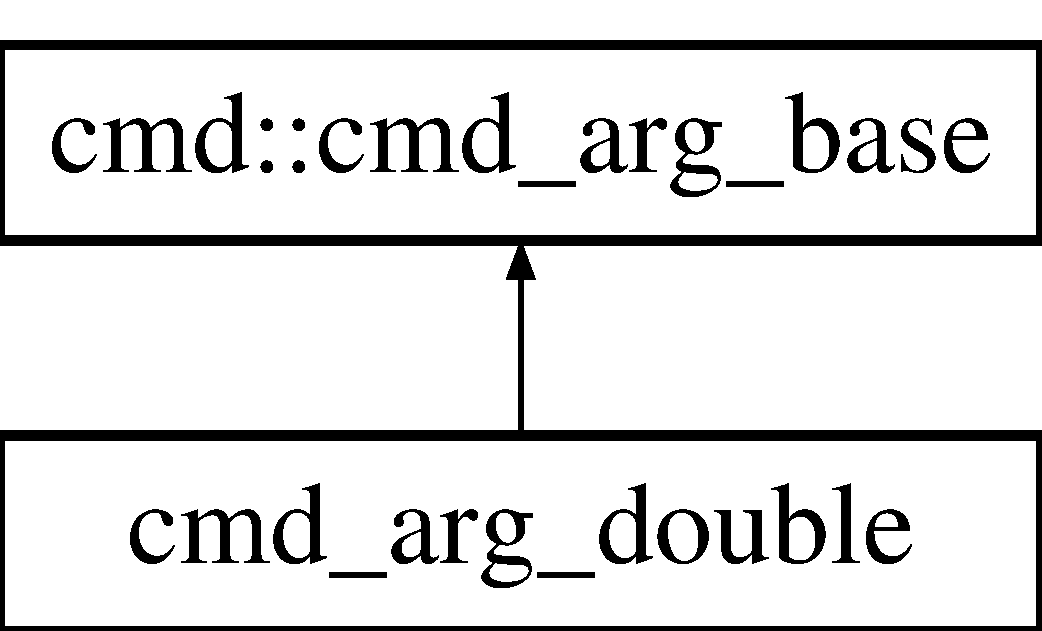
\includegraphics[height=2.000000cm]{classcmd__arg__double}
\end{center}
\end{figure}
\subsection*{Public Member Functions}
\begin{DoxyCompactItemize}
\item 
\hypertarget{classcmd__arg__double_a2b8fcb6d9d4a6f70cfdaf9856df0c2cf}{double \hyperlink{classcmd__arg__double_a2b8fcb6d9d4a6f70cfdaf9856df0c2cf}{get\-\_\-value} () const }\label{classcmd__arg__double_a2b8fcb6d9d4a6f70cfdaf9856df0c2cf}

\begin{DoxyCompactList}\small\item\em Gets double argument's value. \end{DoxyCompactList}\item 
\hypertarget{classcmd__arg__double_a7d419b419af85dfe19e4082b2696eec3}{double \hyperlink{classcmd__arg__double_a7d419b419af85dfe19e4082b2696eec3}{get\-\_\-default\-\_\-value} () const }\label{classcmd__arg__double_a7d419b419af85dfe19e4082b2696eec3}

\begin{DoxyCompactList}\small\item\em Gets double argument's default value. \end{DoxyCompactList}\item 
\hypertarget{classcmd__arg__double_a4b7dc6e7a0520080f456896635eaaa1a}{virtual void \hyperlink{classcmd__arg__double_a4b7dc6e7a0520080f456896635eaaa1a}{set\-\_\-value} (const std\-::string \&v)}\label{classcmd__arg__double_a4b7dc6e7a0520080f456896635eaaa1a}

\begin{DoxyCompactList}\small\item\em Sets double argument's value from string. \end{DoxyCompactList}\item 
\hypertarget{classcmd__arg__double_acdee4ee56f59219be6d8778dd6e84633}{virtual void \hyperlink{classcmd__arg__double_acdee4ee56f59219be6d8778dd6e84633}{reset} ()}\label{classcmd__arg__double_acdee4ee56f59219be6d8778dd6e84633}

\begin{DoxyCompactList}\small\item\em Resets double argument. \end{DoxyCompactList}\item 
\hyperlink{classcmd__arg__double_a41baf85e356cf8807fb1c3011b1f865a}{cmd\-\_\-arg\-\_\-double} (std\-::string name, double default\-\_\-value=false)
\begin{DoxyCompactList}\small\item\em Constructor. \end{DoxyCompactList}\end{DoxyCompactItemize}


\subsection{Detailed Description}
Keeps double command argument. 

\subsection{Constructor \& Destructor Documentation}
\hypertarget{classcmd__arg__double_a41baf85e356cf8807fb1c3011b1f865a}{\index{cmd\-\_\-arg\-\_\-double@{cmd\-\_\-arg\-\_\-double}!cmd\-\_\-arg\-\_\-double@{cmd\-\_\-arg\-\_\-double}}
\index{cmd\-\_\-arg\-\_\-double@{cmd\-\_\-arg\-\_\-double}!cmd_arg_double@{cmd\-\_\-arg\-\_\-double}}
\subsubsection[{cmd\-\_\-arg\-\_\-double}]{\setlength{\rightskip}{0pt plus 5cm}cmd\-\_\-arg\-\_\-double\-::cmd\-\_\-arg\-\_\-double (
\begin{DoxyParamCaption}
\item[{std\-::string}]{name, }
\item[{double}]{default\-\_\-value = {\ttfamily false}}
\end{DoxyParamCaption}
)}}\label{classcmd__arg__double_a41baf85e356cf8807fb1c3011b1f865a}


Constructor. 


\begin{DoxyParams}{Parameters}
{\em name} & Name of double argument. \\
\hline
{\em default\-\_\-value} & Default value. \\
\hline
\end{DoxyParams}


The documentation for this class was generated from the following files\-:\begin{DoxyCompactItemize}
\item 
cmd\-\_\-arg/\hyperlink{cmd__arg__double_8h}{cmd\-\_\-arg\-\_\-double.\-h}\item 
cmd\-\_\-arg/cmd\-\_\-arg\-\_\-double.\-cpp\end{DoxyCompactItemize}

\hypertarget{classcmd__arg__int}{\section{cmd\-\_\-arg\-\_\-int Class Reference}
\label{classcmd__arg__int}\index{cmd\-\_\-arg\-\_\-int@{cmd\-\_\-arg\-\_\-int}}
}


Keeps integer command argument.  




{\ttfamily \#include $<$cmd\-\_\-arg\-\_\-int.\-h$>$}

Inheritance diagram for cmd\-\_\-arg\-\_\-int\-:\begin{figure}[H]
\begin{center}
\leavevmode
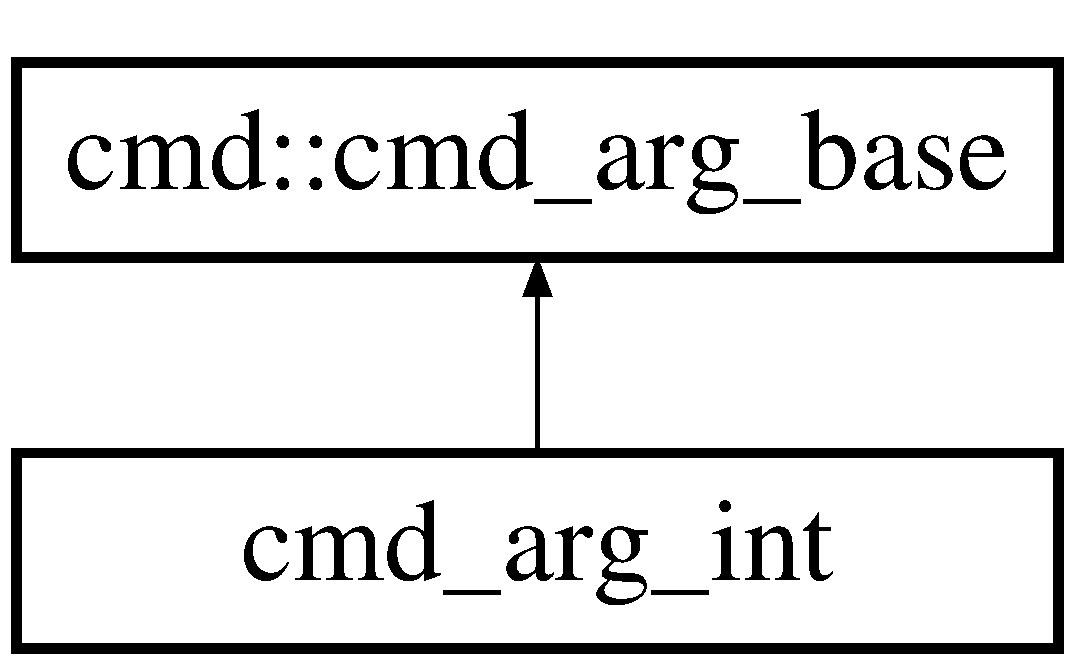
\includegraphics[height=2.000000cm]{classcmd__arg__int}
\end{center}
\end{figure}
\subsection*{Public Member Functions}
\begin{DoxyCompactItemize}
\item 
\hypertarget{classcmd__arg__int_ac2d03f4b0cf2a17ccf0ca60aef0aa403}{int \hyperlink{classcmd__arg__int_ac2d03f4b0cf2a17ccf0ca60aef0aa403}{get\-\_\-value} () const }\label{classcmd__arg__int_ac2d03f4b0cf2a17ccf0ca60aef0aa403}

\begin{DoxyCompactList}\small\item\em Gets integer argument's value. \end{DoxyCompactList}\item 
\hypertarget{classcmd__arg__int_a7e0db1b82dd071fa0ce66e77b9109545}{int \hyperlink{classcmd__arg__int_a7e0db1b82dd071fa0ce66e77b9109545}{get\-\_\-default\-\_\-value} () const }\label{classcmd__arg__int_a7e0db1b82dd071fa0ce66e77b9109545}

\begin{DoxyCompactList}\small\item\em Gets integer argument's default value. \end{DoxyCompactList}\item 
\hypertarget{classcmd__arg__int_a04883e51fb34d7c2e3b9c6b6e3151ad8}{virtual void \hyperlink{classcmd__arg__int_a04883e51fb34d7c2e3b9c6b6e3151ad8}{set\-\_\-value} (const std\-::string \&v)}\label{classcmd__arg__int_a04883e51fb34d7c2e3b9c6b6e3151ad8}

\begin{DoxyCompactList}\small\item\em Sets integer argument's value from string. \end{DoxyCompactList}\item 
\hypertarget{classcmd__arg__int_a97f21fe9b1e529db6fc24754901bdb03}{virtual void \hyperlink{classcmd__arg__int_a97f21fe9b1e529db6fc24754901bdb03}{reset} ()}\label{classcmd__arg__int_a97f21fe9b1e529db6fc24754901bdb03}

\begin{DoxyCompactList}\small\item\em Resets integer argument. \end{DoxyCompactList}\item 
\hyperlink{classcmd__arg__int_a19c0e1b05106ded2c562768cbe1cffe3}{cmd\-\_\-arg\-\_\-int} (std\-::string name, int default\-\_\-value=false)
\begin{DoxyCompactList}\small\item\em Constructor. \end{DoxyCompactList}\end{DoxyCompactItemize}


\subsection{Detailed Description}
Keeps integer command argument. 

\subsection{Constructor \& Destructor Documentation}
\hypertarget{classcmd__arg__int_a19c0e1b05106ded2c562768cbe1cffe3}{\index{cmd\-\_\-arg\-\_\-int@{cmd\-\_\-arg\-\_\-int}!cmd\-\_\-arg\-\_\-int@{cmd\-\_\-arg\-\_\-int}}
\index{cmd\-\_\-arg\-\_\-int@{cmd\-\_\-arg\-\_\-int}!cmd_arg_int@{cmd\-\_\-arg\-\_\-int}}
\subsubsection[{cmd\-\_\-arg\-\_\-int}]{\setlength{\rightskip}{0pt plus 5cm}cmd\-\_\-arg\-\_\-int\-::cmd\-\_\-arg\-\_\-int (
\begin{DoxyParamCaption}
\item[{std\-::string}]{name, }
\item[{int}]{default\-\_\-value = {\ttfamily false}}
\end{DoxyParamCaption}
)}}\label{classcmd__arg__int_a19c0e1b05106ded2c562768cbe1cffe3}


Constructor. 


\begin{DoxyParams}{Parameters}
{\em name} & Name of integer argument. \\
\hline
{\em default\-\_\-value} & Default value. \\
\hline
\end{DoxyParams}


The documentation for this class was generated from the following files\-:\begin{DoxyCompactItemize}
\item 
cmd\-\_\-arg/\hyperlink{cmd__arg__int_8h}{cmd\-\_\-arg\-\_\-int.\-h}\item 
cmd\-\_\-arg/cmd\-\_\-arg\-\_\-int.\-cpp\end{DoxyCompactItemize}

\hypertarget{classcmd__arg__string}{\section{cmd\-\_\-arg\-\_\-string Class Reference}
\label{classcmd__arg__string}\index{cmd\-\_\-arg\-\_\-string@{cmd\-\_\-arg\-\_\-string}}
}


Keeps string command argument.  




{\ttfamily \#include $<$cmd\-\_\-arg\-\_\-string.\-h$>$}

Inheritance diagram for cmd\-\_\-arg\-\_\-string\-:\begin{figure}[H]
\begin{center}
\leavevmode
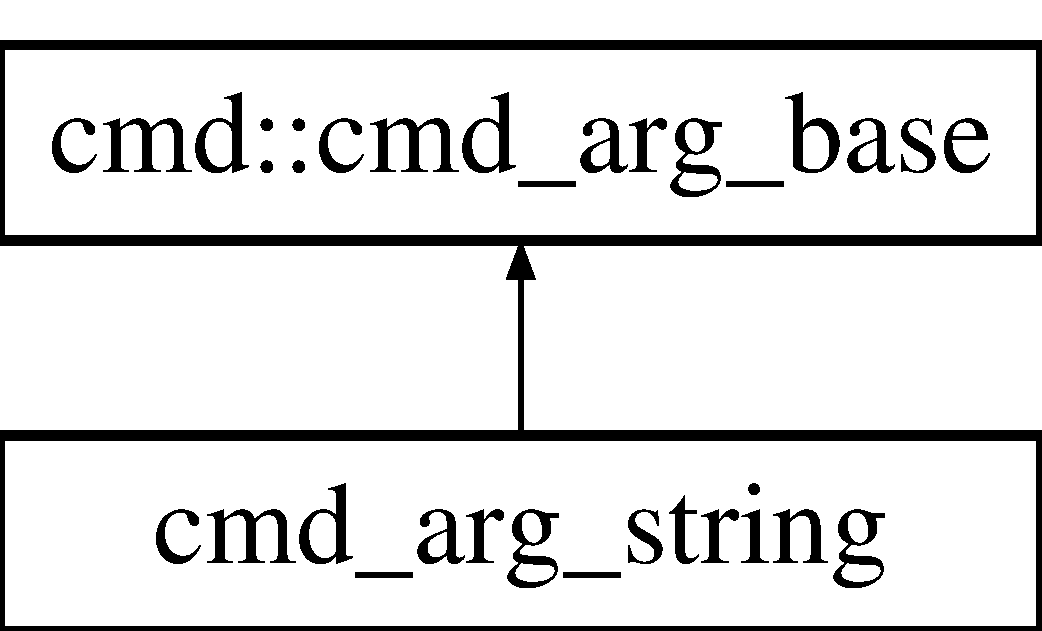
\includegraphics[height=2.000000cm]{classcmd__arg__string}
\end{center}
\end{figure}
\subsection*{Public Member Functions}
\begin{DoxyCompactItemize}
\item 
\hypertarget{classcmd__arg__string_a429f6c147a44c4e89162f194bf96fb2a}{std\-::string \hyperlink{classcmd__arg__string_a429f6c147a44c4e89162f194bf96fb2a}{get\-\_\-value} () const }\label{classcmd__arg__string_a429f6c147a44c4e89162f194bf96fb2a}

\begin{DoxyCompactList}\small\item\em Gets string argument's value. \end{DoxyCompactList}\item 
\hypertarget{classcmd__arg__string_a1bb4bd09605e452c4dd9406bd8d52f16}{std\-::string \hyperlink{classcmd__arg__string_a1bb4bd09605e452c4dd9406bd8d52f16}{get\-\_\-default\-\_\-value} () const }\label{classcmd__arg__string_a1bb4bd09605e452c4dd9406bd8d52f16}

\begin{DoxyCompactList}\small\item\em Gets string argument's default value. \end{DoxyCompactList}\item 
\hypertarget{classcmd__arg__string_a434d6b2a9a6ae7e35043113cc0551140}{virtual void \hyperlink{classcmd__arg__string_a434d6b2a9a6ae7e35043113cc0551140}{set\-\_\-value} (const std\-::string \&v)}\label{classcmd__arg__string_a434d6b2a9a6ae7e35043113cc0551140}

\begin{DoxyCompactList}\small\item\em Sets string argument's value from string. \end{DoxyCompactList}\item 
\hypertarget{classcmd__arg__string_aacc88a0b8b77fc736ae2e475e03bbdcd}{virtual void \hyperlink{classcmd__arg__string_aacc88a0b8b77fc736ae2e475e03bbdcd}{reset} ()}\label{classcmd__arg__string_aacc88a0b8b77fc736ae2e475e03bbdcd}

\begin{DoxyCompactList}\small\item\em Resets string argument. \end{DoxyCompactList}\item 
\hyperlink{classcmd__arg__string_a25dc37fe19abaad0be2bce2a7956c27d}{cmd\-\_\-arg\-\_\-string} (std\-::string name, std\-::string default\-\_\-value=false)
\begin{DoxyCompactList}\small\item\em Constructor. \end{DoxyCompactList}\end{DoxyCompactItemize}


\subsection{Detailed Description}
Keeps string command argument. 

\subsection{Constructor \& Destructor Documentation}
\hypertarget{classcmd__arg__string_a25dc37fe19abaad0be2bce2a7956c27d}{\index{cmd\-\_\-arg\-\_\-string@{cmd\-\_\-arg\-\_\-string}!cmd\-\_\-arg\-\_\-string@{cmd\-\_\-arg\-\_\-string}}
\index{cmd\-\_\-arg\-\_\-string@{cmd\-\_\-arg\-\_\-string}!cmd_arg_string@{cmd\-\_\-arg\-\_\-string}}
\subsubsection[{cmd\-\_\-arg\-\_\-string}]{\setlength{\rightskip}{0pt plus 5cm}cmd\-\_\-arg\-\_\-string\-::cmd\-\_\-arg\-\_\-string (
\begin{DoxyParamCaption}
\item[{std\-::string}]{name, }
\item[{std\-::string}]{default\-\_\-value = {\ttfamily false}}
\end{DoxyParamCaption}
)}}\label{classcmd__arg__string_a25dc37fe19abaad0be2bce2a7956c27d}


Constructor. 


\begin{DoxyParams}{Parameters}
{\em name} & Name of string argument. \\
\hline
{\em default\-\_\-value} & Default value. \\
\hline
\end{DoxyParams}


The documentation for this class was generated from the following files\-:\begin{DoxyCompactItemize}
\item 
cmd\-\_\-arg/\hyperlink{cmd__arg__string_8h}{cmd\-\_\-arg\-\_\-string.\-h}\item 
cmd\-\_\-arg/cmd\-\_\-arg\-\_\-string.\-cpp\end{DoxyCompactItemize}

\hypertarget{classcmd_1_1cmd__base}{\section{cmd\-:\-:cmd\-\_\-base Class Reference}
\label{classcmd_1_1cmd__base}\index{cmd\-::cmd\-\_\-base@{cmd\-::cmd\-\_\-base}}
}


Abstract base class commands.  




{\ttfamily \#include $<$cmd\-\_\-base.\-h$>$}

\subsection*{Public Member Functions}
\begin{DoxyCompactItemize}
\item 
const std\-::string \& \hyperlink{classcmd_1_1cmd__base_a0a2177aba2d3cef3462bfafe3ffaf5b6}{get\-\_\-name} () const 
\begin{DoxyCompactList}\small\item\em Gets command's name. \end{DoxyCompactList}\item 
bool \hyperlink{classcmd_1_1cmd__base_a4e98978dd7eaaaa25bc290a6e9057133}{is\-\_\-equal} (const std\-::string \&n) const 
\begin{DoxyCompactList}\small\item\em Checks if command has same name. \end{DoxyCompactList}\item 
void \hyperlink{classcmd_1_1cmd__base_a4a9946f2ad47ebb8f31907c4069bf63e}{add\-\_\-argument} (\hyperlink{classcmd_1_1cmd__arg__base}{cmd\-\_\-arg\-\_\-base} $\ast$a)
\begin{DoxyCompactList}\small\item\em Adds argument to argument list of command. \end{DoxyCompactList}\item 
void \hyperlink{classcmd_1_1cmd__base_a76d5244c838a19180902422ece888146}{set\-\_\-arg\-\_\-value} (const std\-::string \&arg\-\_\-name, const std\-::string \&arg\-\_\-value)
\begin{DoxyCompactList}\small\item\em Sets arg's value. \end{DoxyCompactList}\item 
\hypertarget{classcmd_1_1cmd__base_ab7f760082a8db20b722ad3db5898f88d}{void \hyperlink{classcmd_1_1cmd__base_ab7f760082a8db20b722ad3db5898f88d}{reset} ()}\label{classcmd_1_1cmd__base_ab7f760082a8db20b722ad3db5898f88d}

\begin{DoxyCompactList}\small\item\em Resets all argumets of command. \end{DoxyCompactList}\item 
\hypertarget{classcmd_1_1cmd__base_a61a0557f1380b4dd7f98458b119aae7c}{virtual void \hyperlink{classcmd_1_1cmd__base_a61a0557f1380b4dd7f98458b119aae7c}{execute} ()=0}\label{classcmd_1_1cmd__base_a61a0557f1380b4dd7f98458b119aae7c}

\begin{DoxyCompactList}\small\item\em pure virtual function to make execution of command. \end{DoxyCompactList}\item 
\hyperlink{classcmd_1_1cmd__base_aef539046901d74b2499f83fe7eeb178e}{cmd\-\_\-base} (const std\-::string \&name)
\begin{DoxyCompactList}\small\item\em Constructor. \end{DoxyCompactList}\item 
\hypertarget{classcmd_1_1cmd__base_a2d68b12de6b8e4d5ef4ede6a63f33ed2}{\hyperlink{classcmd_1_1cmd__base_a2d68b12de6b8e4d5ef4ede6a63f33ed2}{$\sim$cmd\-\_\-base} ()}\label{classcmd_1_1cmd__base_a2d68b12de6b8e4d5ef4ede6a63f33ed2}

\begin{DoxyCompactList}\small\item\em Virtual destructor. \end{DoxyCompactList}\end{DoxyCompactItemize}


\subsection{Detailed Description}
Abstract base class commands. 

\subsection{Constructor \& Destructor Documentation}
\hypertarget{classcmd_1_1cmd__base_aef539046901d74b2499f83fe7eeb178e}{\index{cmd\-::cmd\-\_\-base@{cmd\-::cmd\-\_\-base}!cmd\-\_\-base@{cmd\-\_\-base}}
\index{cmd\-\_\-base@{cmd\-\_\-base}!cmd::cmd_base@{cmd\-::cmd\-\_\-base}}
\subsubsection[{cmd\-\_\-base}]{\setlength{\rightskip}{0pt plus 5cm}cmd\-::cmd\-\_\-base\-::cmd\-\_\-base (
\begin{DoxyParamCaption}
\item[{const std\-::string \&}]{name}
\end{DoxyParamCaption}
)}}\label{classcmd_1_1cmd__base_aef539046901d74b2499f83fe7eeb178e}


Constructor. 


\begin{DoxyParams}{Parameters}
{\em name} & Name of command. \\
\hline
\end{DoxyParams}


\subsection{Member Function Documentation}
\hypertarget{classcmd_1_1cmd__base_a4a9946f2ad47ebb8f31907c4069bf63e}{\index{cmd\-::cmd\-\_\-base@{cmd\-::cmd\-\_\-base}!add\-\_\-argument@{add\-\_\-argument}}
\index{add\-\_\-argument@{add\-\_\-argument}!cmd::cmd_base@{cmd\-::cmd\-\_\-base}}
\subsubsection[{add\-\_\-argument}]{\setlength{\rightskip}{0pt plus 5cm}void cmd\-::cmd\-\_\-base\-::add\-\_\-argument (
\begin{DoxyParamCaption}
\item[{{\bf cmd\-\_\-arg\-\_\-base} $\ast$}]{a}
\end{DoxyParamCaption}
)}}\label{classcmd_1_1cmd__base_a4a9946f2ad47ebb8f31907c4069bf63e}


Adds argument to argument list of command. 


\begin{DoxyParams}{Parameters}
{\em a} & Argument to add. \\
\hline
\end{DoxyParams}
\hypertarget{classcmd_1_1cmd__base_a0a2177aba2d3cef3462bfafe3ffaf5b6}{\index{cmd\-::cmd\-\_\-base@{cmd\-::cmd\-\_\-base}!get\-\_\-name@{get\-\_\-name}}
\index{get\-\_\-name@{get\-\_\-name}!cmd::cmd_base@{cmd\-::cmd\-\_\-base}}
\subsubsection[{get\-\_\-name}]{\setlength{\rightskip}{0pt plus 5cm}const std\-::string \& cmd\-::cmd\-\_\-base\-::get\-\_\-name (
\begin{DoxyParamCaption}
{}
\end{DoxyParamCaption}
) const}}\label{classcmd_1_1cmd__base_a0a2177aba2d3cef3462bfafe3ffaf5b6}


Gets command's name. 

\begin{DoxyReturn}{Returns}
Constant access to command's name. 
\end{DoxyReturn}
\hypertarget{classcmd_1_1cmd__base_a4e98978dd7eaaaa25bc290a6e9057133}{\index{cmd\-::cmd\-\_\-base@{cmd\-::cmd\-\_\-base}!is\-\_\-equal@{is\-\_\-equal}}
\index{is\-\_\-equal@{is\-\_\-equal}!cmd::cmd_base@{cmd\-::cmd\-\_\-base}}
\subsubsection[{is\-\_\-equal}]{\setlength{\rightskip}{0pt plus 5cm}bool cmd\-::cmd\-\_\-base\-::is\-\_\-equal (
\begin{DoxyParamCaption}
\item[{const std\-::string \&}]{n}
\end{DoxyParamCaption}
) const}}\label{classcmd_1_1cmd__base_a4e98978dd7eaaaa25bc290a6e9057133}


Checks if command has same name. 


\begin{DoxyParams}{Parameters}
{\em n} & Name to compare. \\
\hline
\end{DoxyParams}
\begin{DoxyReturn}{Returns}
true if argument's name is equal to the given name. 
\end{DoxyReturn}
\hypertarget{classcmd_1_1cmd__base_a76d5244c838a19180902422ece888146}{\index{cmd\-::cmd\-\_\-base@{cmd\-::cmd\-\_\-base}!set\-\_\-arg\-\_\-value@{set\-\_\-arg\-\_\-value}}
\index{set\-\_\-arg\-\_\-value@{set\-\_\-arg\-\_\-value}!cmd::cmd_base@{cmd\-::cmd\-\_\-base}}
\subsubsection[{set\-\_\-arg\-\_\-value}]{\setlength{\rightskip}{0pt plus 5cm}void cmd\-::cmd\-\_\-base\-::set\-\_\-arg\-\_\-value (
\begin{DoxyParamCaption}
\item[{const std\-::string \&}]{arg\-\_\-name, }
\item[{const std\-::string \&}]{arg\-\_\-value}
\end{DoxyParamCaption}
)}}\label{classcmd_1_1cmd__base_a76d5244c838a19180902422ece888146}


Sets arg's value. 


\begin{DoxyParams}{Parameters}
{\em arg\-\_\-name} & Name of argument to be set. \\
\hline
{\em arg\-\_\-value} & Value to set. \\
\hline
\end{DoxyParams}


The documentation for this class was generated from the following files\-:\begin{DoxyCompactItemize}
\item 
cmd\-\_\-base/\hyperlink{cmd__base_8h}{cmd\-\_\-base.\-h}\item 
cmd\-\_\-base/\hyperlink{cmd__base_8cpp}{cmd\-\_\-base.\-cpp}\end{DoxyCompactItemize}

\hypertarget{classcmd_1_1cmd__processor}{\section{cmd\-:\-:cmd\-\_\-processor Class Reference}
\label{classcmd_1_1cmd__processor}\index{cmd\-::cmd\-\_\-processor@{cmd\-::cmd\-\_\-processor}}
}


Central singleton class for processing command line entries.  




{\ttfamily \#include $<$cmd\-\_\-processor.\-h$>$}

\subsection*{command management.}
\begin{DoxyCompactItemize}
\item 
void \hyperlink{classcmd_1_1cmd__processor_a03712564937c37f196633880f8876a3a}{add\-\_\-command} (\hyperlink{classcmd_1_1cmd__base}{cmd\-\_\-base} $\ast$cmd)
\begin{DoxyCompactList}\small\item\em Adds command to command list of command processor. \end{DoxyCompactList}\item 
void \hyperlink{classcmd_1_1cmd__processor_a03ac466a41a77fc30490ae72446c6e2d}{parse\-\_\-and\-\_\-execute\-\_\-command} (const std\-::string \&c\-\_\-l)
\begin{DoxyCompactList}\small\item\em Parses command string and makes execution. \end{DoxyCompactList}\end{DoxyCompactItemize}
\subsection*{singleton management}
\begin{DoxyCompactItemize}
\item 
\hypertarget{classcmd_1_1cmd__processor_a469ef9311a2c4dacd99172acd9568004}{static \hyperlink{classcmd_1_1cmd__processor}{cmd\-\_\-processor} \& \hyperlink{classcmd_1_1cmd__processor_a469ef9311a2c4dacd99172acd9568004}{get\-\_\-instance} ()}\label{classcmd_1_1cmd__processor_a469ef9311a2c4dacd99172acd9568004}

\begin{DoxyCompactList}\small\item\em Gets singletone object. \end{DoxyCompactList}\item 
\hypertarget{classcmd_1_1cmd__processor_af1575ac253ee9b68a0f90fb1151635a8}{static void \hyperlink{classcmd_1_1cmd__processor_af1575ac253ee9b68a0f90fb1151635a8}{instantiate} ()}\label{classcmd_1_1cmd__processor_af1575ac253ee9b68a0f90fb1151635a8}

\begin{DoxyCompactList}\small\item\em Intstantiates singletone object. \end{DoxyCompactList}\item 
\hypertarget{classcmd_1_1cmd__processor_a5cfe052f862135f78149afcfbb822fbd}{static void \hyperlink{classcmd_1_1cmd__processor_a5cfe052f862135f78149afcfbb822fbd}{destroy} ()}\label{classcmd_1_1cmd__processor_a5cfe052f862135f78149afcfbb822fbd}

\begin{DoxyCompactList}\small\item\em Destroys singletone object. \end{DoxyCompactList}\end{DoxyCompactItemize}
\subsection*{Special member functions.}
\begin{DoxyCompactItemize}
\item 
\hypertarget{classcmd_1_1cmd__processor_a43ff9a70dcb3b5f13e64aa03b0f2953f}{\hyperlink{classcmd_1_1cmd__processor_a43ff9a70dcb3b5f13e64aa03b0f2953f}{cmd\-\_\-processor} ()=default}\label{classcmd_1_1cmd__processor_a43ff9a70dcb3b5f13e64aa03b0f2953f}

\begin{DoxyCompactList}\small\item\em Constructor. \end{DoxyCompactList}\item 
\hypertarget{classcmd_1_1cmd__processor_a50b3836ac227c968d04d8aec461e1cb7}{\hyperlink{classcmd_1_1cmd__processor_a50b3836ac227c968d04d8aec461e1cb7}{$\sim$cmd\-\_\-processor} ()}\label{classcmd_1_1cmd__processor_a50b3836ac227c968d04d8aec461e1cb7}

\begin{DoxyCompactList}\small\item\em Destructor. \end{DoxyCompactList}\end{DoxyCompactItemize}


\subsection{Detailed Description}
Central singleton class for processing command line entries. 

\subsection{Member Function Documentation}
\hypertarget{classcmd_1_1cmd__processor_a03712564937c37f196633880f8876a3a}{\index{cmd\-::cmd\-\_\-processor@{cmd\-::cmd\-\_\-processor}!add\-\_\-command@{add\-\_\-command}}
\index{add\-\_\-command@{add\-\_\-command}!cmd::cmd_processor@{cmd\-::cmd\-\_\-processor}}
\subsubsection[{add\-\_\-command}]{\setlength{\rightskip}{0pt plus 5cm}void cmd\-::cmd\-\_\-processor\-::add\-\_\-command (
\begin{DoxyParamCaption}
\item[{{\bf cmd\-\_\-base} $\ast$}]{cmd}
\end{DoxyParamCaption}
)}}\label{classcmd_1_1cmd__processor_a03712564937c37f196633880f8876a3a}


Adds command to command list of command processor. 


\begin{DoxyParams}{Parameters}
{\em cmd} & Command to add. \\
\hline
\end{DoxyParams}
\hypertarget{classcmd_1_1cmd__processor_a03ac466a41a77fc30490ae72446c6e2d}{\index{cmd\-::cmd\-\_\-processor@{cmd\-::cmd\-\_\-processor}!parse\-\_\-and\-\_\-execute\-\_\-command@{parse\-\_\-and\-\_\-execute\-\_\-command}}
\index{parse\-\_\-and\-\_\-execute\-\_\-command@{parse\-\_\-and\-\_\-execute\-\_\-command}!cmd::cmd_processor@{cmd\-::cmd\-\_\-processor}}
\subsubsection[{parse\-\_\-and\-\_\-execute\-\_\-command}]{\setlength{\rightskip}{0pt plus 5cm}void cmd\-::cmd\-\_\-processor\-::parse\-\_\-and\-\_\-execute\-\_\-command (
\begin{DoxyParamCaption}
\item[{const std\-::string \&}]{c\-\_\-l}
\end{DoxyParamCaption}
)}}\label{classcmd_1_1cmd__processor_a03ac466a41a77fc30490ae72446c6e2d}


Parses command string and makes execution. 


\begin{DoxyParams}{Parameters}
{\em c\-\_\-l} & Command string. \\
\hline
\end{DoxyParams}


The documentation for this class was generated from the following files\-:\begin{DoxyCompactItemize}
\item 
cmd\-\_\-processor/\hyperlink{cmd__processor_8h}{cmd\-\_\-processor.\-h}\item 
cmd\-\_\-processor/\hyperlink{cmd__processor_8cpp}{cmd\-\_\-processor.\-cpp}\end{DoxyCompactItemize}

\hypertarget{classcmd_1_1exception}{\section{cmd\-:\-:exception Class Reference}
\label{classcmd_1_1exception}\index{cmd\-::exception@{cmd\-::exception}}
}


exception system for cmd level exceptions.  




{\ttfamily \#include $<$cmd\-\_\-exception.\-h$>$}

\subsection*{Public Member Functions}
\begin{DoxyCompactItemize}
\item 
\hypertarget{classcmd_1_1exception_a432688fc0fe4b5db880caee4cdccf521}{const std\-::string \& \hyperlink{classcmd_1_1exception_a432688fc0fe4b5db880caee4cdccf521}{get\-\_\-message} () const }\label{classcmd_1_1exception_a432688fc0fe4b5db880caee4cdccf521}

\begin{DoxyCompactList}\small\item\em Gets message of exception. \end{DoxyCompactList}\item 
\hyperlink{classcmd_1_1exception_a88d53316e2e387daa22889d2be7fb641}{exception} (const std\-::string \&m)
\begin{DoxyCompactList}\small\item\em Constructor. \end{DoxyCompactList}\item 
\hypertarget{classcmd_1_1exception_afa9a99039e2fd9b110b466e2a2e03613}{virtual \hyperlink{classcmd_1_1exception_afa9a99039e2fd9b110b466e2a2e03613}{$\sim$exception} ()}\label{classcmd_1_1exception_afa9a99039e2fd9b110b466e2a2e03613}

\begin{DoxyCompactList}\small\item\em Virtual Destructor. \end{DoxyCompactList}\end{DoxyCompactItemize}


\subsection{Detailed Description}
exception system for cmd level exceptions. 

\subsection{Constructor \& Destructor Documentation}
\hypertarget{classcmd_1_1exception_a88d53316e2e387daa22889d2be7fb641}{\index{cmd\-::exception@{cmd\-::exception}!exception@{exception}}
\index{exception@{exception}!cmd::exception@{cmd\-::exception}}
\subsubsection[{exception}]{\setlength{\rightskip}{0pt plus 5cm}cmd\-::exception\-::exception (
\begin{DoxyParamCaption}
\item[{const std\-::string \&}]{m}
\end{DoxyParamCaption}
)}}\label{classcmd_1_1exception_a88d53316e2e387daa22889d2be7fb641}


Constructor. 


\begin{DoxyParams}{Parameters}
{\em m} & Message of exception. \\
\hline
\end{DoxyParams}


The documentation for this class was generated from the following files\-:\begin{DoxyCompactItemize}
\item 
exceptions/\hyperlink{cmd__exception_8h}{cmd\-\_\-exception.\-h}\item 
exceptions/\hyperlink{cmd__exception_8cpp}{cmd\-\_\-exception.\-cpp}\end{DoxyCompactItemize}

\chapter{File Documentation}
\hypertarget{cmd__arg__bool_8h}{\section{cmd\-\_\-arg/cmd\-\_\-arg\-\_\-bool.h File Reference}
\label{cmd__arg__bool_8h}\index{cmd\-\_\-arg/cmd\-\_\-arg\-\_\-bool.\-h@{cmd\-\_\-arg/cmd\-\_\-arg\-\_\-bool.\-h}}
}


definition of class \hyperlink{classcmd__arg__bool}{cmd\-\_\-arg\-\_\-bool}  


{\ttfamily \#include \char`\"{}cmd\-\_\-arg\-\_\-base.\-h\char`\"{}}\\*
\subsection*{Classes}
\begin{DoxyCompactItemize}
\item 
class \hyperlink{classcmd__arg__bool}{cmd\-\_\-arg\-\_\-bool}
\begin{DoxyCompactList}\small\item\em Keeps boolean command argument. \end{DoxyCompactList}\end{DoxyCompactItemize}


\subsection{Detailed Description}
definition of class \hyperlink{classcmd__arg__bool}{cmd\-\_\-arg\-\_\-bool} declaration of class \hyperlink{classcmd__arg__bool}{cmd\-\_\-arg\-\_\-bool}

\begin{DoxyAuthor}{Author}
Hayk Khachatryan 
\end{DoxyAuthor}

\hypertarget{cmd__arg__double_8h}{\section{cmd\-\_\-arg/cmd\-\_\-arg\-\_\-double.h File Reference}
\label{cmd__arg__double_8h}\index{cmd\-\_\-arg/cmd\-\_\-arg\-\_\-double.\-h@{cmd\-\_\-arg/cmd\-\_\-arg\-\_\-double.\-h}}
}


definition of class \hyperlink{classcmd__arg__double}{cmd\-\_\-arg\-\_\-double}  


{\ttfamily \#include \char`\"{}cmd\-\_\-arg\-\_\-base.\-h\char`\"{}}\\*
\subsection*{Classes}
\begin{DoxyCompactItemize}
\item 
class \hyperlink{classcmd__arg__double}{cmd\-\_\-arg\-\_\-double}
\begin{DoxyCompactList}\small\item\em Keeps double command argument. \end{DoxyCompactList}\end{DoxyCompactItemize}


\subsection{Detailed Description}
definition of class \hyperlink{classcmd__arg__double}{cmd\-\_\-arg\-\_\-double} declaration of class \hyperlink{classcmd__arg__double}{cmd\-\_\-arg\-\_\-double}

\begin{DoxyAuthor}{Author}
Hayk Khachatryan 
\end{DoxyAuthor}

\hypertarget{cmd__arg__int_8h}{\section{cmd\-\_\-arg/cmd\-\_\-arg\-\_\-int.h File Reference}
\label{cmd__arg__int_8h}\index{cmd\-\_\-arg/cmd\-\_\-arg\-\_\-int.\-h@{cmd\-\_\-arg/cmd\-\_\-arg\-\_\-int.\-h}}
}


definition of class \hyperlink{classcmd__arg__int}{cmd\-\_\-arg\-\_\-int}  


{\ttfamily \#include \char`\"{}cmd\-\_\-arg\-\_\-base.\-h\char`\"{}}\\*
\subsection*{Classes}
\begin{DoxyCompactItemize}
\item 
class \hyperlink{classcmd__arg__int}{cmd\-\_\-arg\-\_\-int}
\begin{DoxyCompactList}\small\item\em Keeps integer command argument. \end{DoxyCompactList}\end{DoxyCompactItemize}


\subsection{Detailed Description}
definition of class \hyperlink{classcmd__arg__int}{cmd\-\_\-arg\-\_\-int} declaration of class \hyperlink{classcmd__arg__int}{cmd\-\_\-arg\-\_\-int}

\begin{DoxyAuthor}{Author}
Hayk Khachatryan 
\end{DoxyAuthor}

\hypertarget{cmd__arg__string_8h}{\section{cmd\-\_\-arg/cmd\-\_\-arg\-\_\-string.h File Reference}
\label{cmd__arg__string_8h}\index{cmd\-\_\-arg/cmd\-\_\-arg\-\_\-string.\-h@{cmd\-\_\-arg/cmd\-\_\-arg\-\_\-string.\-h}}
}


definition of class \hyperlink{classcmd__arg__string}{cmd\-\_\-arg\-\_\-string}  


{\ttfamily \#include \char`\"{}cmd\-\_\-arg\-\_\-base.\-h\char`\"{}}\\*
\subsection*{Classes}
\begin{DoxyCompactItemize}
\item 
class \hyperlink{classcmd__arg__string}{cmd\-\_\-arg\-\_\-string}
\begin{DoxyCompactList}\small\item\em Keeps string command argument. \end{DoxyCompactList}\end{DoxyCompactItemize}


\subsection{Detailed Description}
definition of class \hyperlink{classcmd__arg__string}{cmd\-\_\-arg\-\_\-string} declaration of class \hyperlink{classcmd__arg__string}{cmd\-\_\-arg\-\_\-string}

\begin{DoxyAuthor}{Author}
Hayk Khachatryan 
\end{DoxyAuthor}

\hypertarget{cmd__arg__base_8cpp}{\section{cmd\-\_\-base/cmd\-\_\-arg\-\_\-base.cpp File Reference}
\label{cmd__arg__base_8cpp}\index{cmd\-\_\-base/cmd\-\_\-arg\-\_\-base.\-cpp@{cmd\-\_\-base/cmd\-\_\-arg\-\_\-base.\-cpp}}
}


definition of class cmd\-\_\-arg\-\_\-base  


{\ttfamily \#include \char`\"{}cmd\-\_\-arg\-\_\-base.\-h\char`\"{}}\\*
{\ttfamily \#include $<$assert.\-h$>$}\\*
\subsection*{Namespaces}
\begin{DoxyCompactItemize}
\item 
namespace \hyperlink{namespacecmd}{cmd}
\begin{DoxyCompactList}\small\item\em command infrastructure namespace \end{DoxyCompactList}\end{DoxyCompactItemize}


\subsection{Detailed Description}
definition of class cmd\-\_\-arg\-\_\-base \begin{DoxyAuthor}{Author}
Hayk Khachatryan 
\end{DoxyAuthor}

\hypertarget{cmd__arg__base_8h}{\section{cmd\-\_\-base/cmd\-\_\-arg\-\_\-base.h File Reference}
\label{cmd__arg__base_8h}\index{cmd\-\_\-base/cmd\-\_\-arg\-\_\-base.\-h@{cmd\-\_\-base/cmd\-\_\-arg\-\_\-base.\-h}}
}


declaration of class cmd\-\_\-arg\-\_\-base  


{\ttfamily \#include $<$string$>$}\\*
\subsection*{Classes}
\begin{DoxyCompactItemize}
\item 
class \hyperlink{classcmd_1_1cmd__arg__base}{cmd\-::cmd\-\_\-arg\-\_\-base}
\begin{DoxyCompactList}\small\item\em Abstract base class for command args. \end{DoxyCompactList}\end{DoxyCompactItemize}
\subsection*{Namespaces}
\begin{DoxyCompactItemize}
\item 
namespace \hyperlink{namespacecmd}{cmd}
\begin{DoxyCompactList}\small\item\em command infrastructure namespace \end{DoxyCompactList}\end{DoxyCompactItemize}


\subsection{Detailed Description}
declaration of class cmd\-\_\-arg\-\_\-base \begin{DoxyAuthor}{Author}
Hayk Khachatryan 
\end{DoxyAuthor}

\hypertarget{cmd__base_8cpp}{\section{cmd\-\_\-base/cmd\-\_\-base.cpp File Reference}
\label{cmd__base_8cpp}\index{cmd\-\_\-base/cmd\-\_\-base.\-cpp@{cmd\-\_\-base/cmd\-\_\-base.\-cpp}}
}


definition of class cmd\-\_\-base  


{\ttfamily \#include \char`\"{}cmd\-\_\-base.\-h\char`\"{}}\\*
{\ttfamily \#include \char`\"{}cmd\-\_\-arg\-\_\-base.\-h\char`\"{}}\\*
{\ttfamily \#include \char`\"{}cmd\-\_\-exception.\-h\char`\"{}}\\*
{\ttfamily \#include $<$assert.\-h$>$}\\*
\subsection*{Namespaces}
\begin{DoxyCompactItemize}
\item 
namespace \hyperlink{namespacecmd}{cmd}
\begin{DoxyCompactList}\small\item\em command infrastructure namespace \end{DoxyCompactList}\end{DoxyCompactItemize}


\subsection{Detailed Description}
definition of class cmd\-\_\-base \begin{DoxyAuthor}{Author}
Hayk Khachatryan 
\end{DoxyAuthor}

\hypertarget{cmd__base_8h}{\section{cmd\-\_\-base/cmd\-\_\-base.h File Reference}
\label{cmd__base_8h}\index{cmd\-\_\-base/cmd\-\_\-base.\-h@{cmd\-\_\-base/cmd\-\_\-base.\-h}}
}


declaration of class cmd\-\_\-base  


{\ttfamily \#include $<$string$>$}\\*
{\ttfamily \#include $<$map$>$}\\*
\subsection*{Classes}
\begin{DoxyCompactItemize}
\item 
class \hyperlink{classcmd_1_1cmd__base}{cmd\-::cmd\-\_\-base}
\begin{DoxyCompactList}\small\item\em Abstract base class commands. \end{DoxyCompactList}\end{DoxyCompactItemize}
\subsection*{Namespaces}
\begin{DoxyCompactItemize}
\item 
namespace \hyperlink{namespacecmd}{cmd}
\begin{DoxyCompactList}\small\item\em command infrastructure namespace \end{DoxyCompactList}\end{DoxyCompactItemize}


\subsection{Detailed Description}
declaration of class cmd\-\_\-base \begin{DoxyAuthor}{Author}
Hayk Khachatryan 
\end{DoxyAuthor}

\hypertarget{cmd__processor_8cpp}{\section{cmd\-\_\-processor/cmd\-\_\-processor.cpp File Reference}
\label{cmd__processor_8cpp}\index{cmd\-\_\-processor/cmd\-\_\-processor.\-cpp@{cmd\-\_\-processor/cmd\-\_\-processor.\-cpp}}
}


definition of class cmd\-\_\-processor  


{\ttfamily \#include \char`\"{}cmd\-\_\-processor.\-h\char`\"{}}\\*
{\ttfamily \#include \char`\"{}cmd\-\_\-base.\-h\char`\"{}}\\*
{\ttfamily \#include \char`\"{}cmd\-\_\-exception.\-h\char`\"{}}\\*
{\ttfamily \#include $<$assert.\-h$>$}\\*
\subsection*{Namespaces}
\begin{DoxyCompactItemize}
\item 
namespace \hyperlink{namespacecmd}{cmd}
\begin{DoxyCompactList}\small\item\em command infrastructure namespace \end{DoxyCompactList}\end{DoxyCompactItemize}


\subsection{Detailed Description}
definition of class cmd\-\_\-processor \begin{DoxyAuthor}{Author}
Hayk Khachatryan 
\end{DoxyAuthor}

\hypertarget{cmd__processor_8h}{\section{cmd\-\_\-processor/cmd\-\_\-processor.h File Reference}
\label{cmd__processor_8h}\index{cmd\-\_\-processor/cmd\-\_\-processor.\-h@{cmd\-\_\-processor/cmd\-\_\-processor.\-h}}
}


declaration of class cmd\-\_\-processor  


{\ttfamily \#include $<$string$>$}\\*
{\ttfamily \#include $<$map$>$}\\*
{\ttfamily \#include $<$vector$>$}\\*
\subsection*{Classes}
\begin{DoxyCompactItemize}
\item 
class \hyperlink{classcmd_1_1cmd__processor}{cmd\-::cmd\-\_\-processor}
\begin{DoxyCompactList}\small\item\em Central singleton class for processing command line entries. \end{DoxyCompactList}\end{DoxyCompactItemize}
\subsection*{Namespaces}
\begin{DoxyCompactItemize}
\item 
namespace \hyperlink{namespacecmd}{cmd}
\begin{DoxyCompactList}\small\item\em command infrastructure namespace \end{DoxyCompactList}\end{DoxyCompactItemize}


\subsection{Detailed Description}
declaration of class cmd\-\_\-processor \begin{DoxyAuthor}{Author}
Hayk Khachatryan 
\end{DoxyAuthor}

\hypertarget{cmd__exception_8cpp}{\section{exceptions/cmd\-\_\-exception.cpp File Reference}
\label{cmd__exception_8cpp}\index{exceptions/cmd\-\_\-exception.\-cpp@{exceptions/cmd\-\_\-exception.\-cpp}}
}


definition of class exception  


{\ttfamily \#include \char`\"{}cmd\-\_\-exception.\-h\char`\"{}}\\*
{\ttfamily \#include $<$assert.\-h$>$}\\*
\subsection*{Namespaces}
\begin{DoxyCompactItemize}
\item 
namespace \hyperlink{namespacecmd}{cmd}
\begin{DoxyCompactList}\small\item\em command infrastructure namespace \end{DoxyCompactList}\end{DoxyCompactItemize}


\subsection{Detailed Description}
definition of class exception \begin{DoxyAuthor}{Author}
Hayk Khachatryan 
\end{DoxyAuthor}

\hypertarget{cmd__exception_8h}{\section{exceptions/cmd\-\_\-exception.h File Reference}
\label{cmd__exception_8h}\index{exceptions/cmd\-\_\-exception.\-h@{exceptions/cmd\-\_\-exception.\-h}}
}


declaration of class exception  


{\ttfamily \#include $<$string$>$}\\*
\subsection*{Classes}
\begin{DoxyCompactItemize}
\item 
class \hyperlink{classcmd_1_1exception}{cmd\-::exception}
\begin{DoxyCompactList}\small\item\em exception system for cmd level exceptions. \end{DoxyCompactList}\end{DoxyCompactItemize}
\subsection*{Namespaces}
\begin{DoxyCompactItemize}
\item 
namespace \hyperlink{namespacecmd}{cmd}
\begin{DoxyCompactList}\small\item\em command infrastructure namespace \end{DoxyCompactList}\end{DoxyCompactItemize}


\subsection{Detailed Description}
declaration of class exception \begin{DoxyAuthor}{Author}
Hayk Khachatryan 
\end{DoxyAuthor}

\hypertarget{central__engine_8cpp}{\section{main/central\-\_\-engine.cpp File Reference}
\label{central__engine_8cpp}\index{main/central\-\_\-engine.\-cpp@{main/central\-\_\-engine.\-cpp}}
}


definition of class \hyperlink{classcentral__engine}{central\-\_\-engine}  


{\ttfamily \#include \char`\"{}central\-\_\-engine.\-h\char`\"{}}\\*
{\ttfamily \#include \char`\"{}cmd\-\_\-processor.\-h\char`\"{}}\\*
{\ttfamily \#include \char`\"{}cmd\-\_\-exception.\-h\char`\"{}}\\*
{\ttfamily \#include $<$iostream$>$}\\*
{\ttfamily \#include $<$assert.\-h$>$}\\*


\subsection{Detailed Description}
definition of class \hyperlink{classcentral__engine}{central\-\_\-engine} \begin{DoxyAuthor}{Author}
Hayk Khachatryan 
\end{DoxyAuthor}

\hypertarget{central__engine_8h}{\section{main/central\-\_\-engine.h File Reference}
\label{central__engine_8h}\index{main/central\-\_\-engine.\-h@{main/central\-\_\-engine.\-h}}
}


declaration of class \hyperlink{classcentral__engine}{central\-\_\-engine}  


\subsection*{Classes}
\begin{DoxyCompactItemize}
\item 
class \hyperlink{classcentral__engine}{central\-\_\-engine}
\begin{DoxyCompactList}\small\item\em Central engine to handle program initialization, uninitialization, command-\/line, e.\-t.\-c. \end{DoxyCompactList}\end{DoxyCompactItemize}


\subsection{Detailed Description}
declaration of class \hyperlink{classcentral__engine}{central\-\_\-engine} \begin{DoxyAuthor}{Author}
Hayk Khachatryan 
\end{DoxyAuthor}

\addcontentsline{toc}{part}{Index}
\printindex
\end{document}
